% Created by tikzDevice version 0.6.1 on 2011-07-24 13:32:06
% !TEX encoding = UTF-8 Unicode
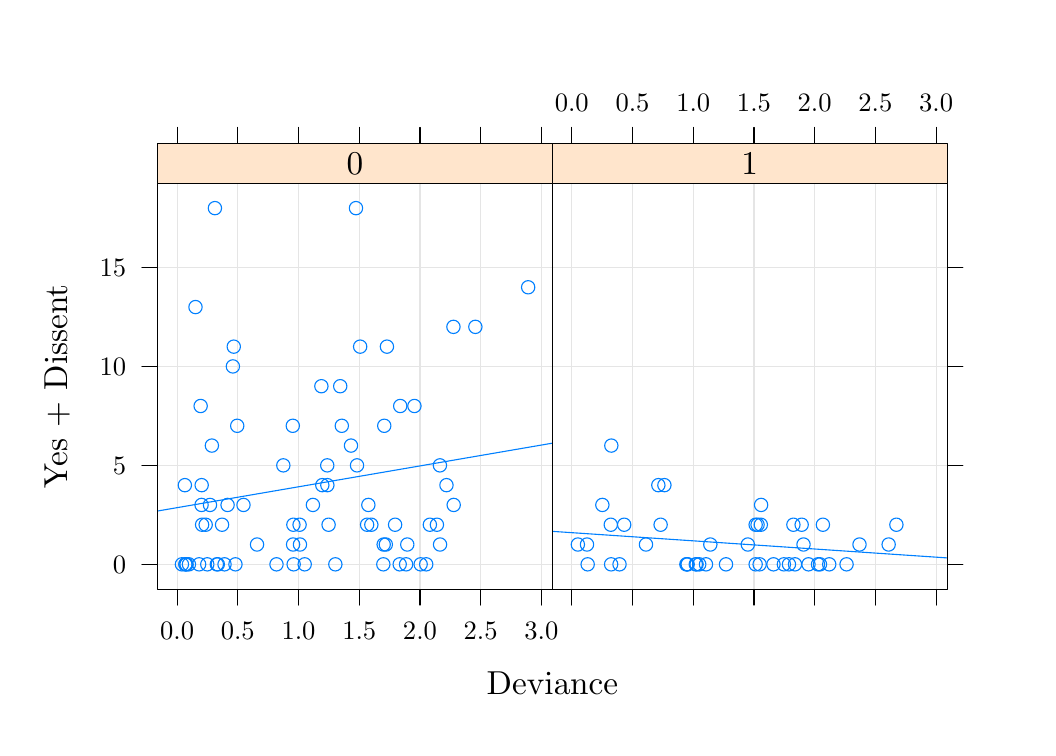
\begin{tikzpicture}[x=1pt,y=1pt]
\definecolor[named]{drawColor}{rgb}{0.00,0.00,0.00}
\definecolor[named]{fillColor}{rgb}{1.00,1.00,1.00}
\fill[color=fillColor,] (0,0) rectangle (361.35,252.94);
\begin{scope}
\path[clip] (  0.00,  0.00) rectangle (361.35,252.94);
\end{scope}
\begin{scope}
\path[clip] (  0.00,  0.00) rectangle (361.35,252.94);

\draw[fill opacity=0.00,draw opacity=0.00,] (  0.00,  0.00) rectangle (361.35,252.94);
\definecolor[named]{drawColor}{rgb}{0.00,0.00,0.00}

\node[color=drawColor,anchor=base,inner sep=0pt, outer sep=0pt, scale=  1.20] at (189.61, 12.04) {Deviance%
};
\end{scope}
\begin{scope}
\path[clip] (  0.00,  0.00) rectangle (361.35,252.94);
\definecolor[named]{drawColor}{rgb}{0.00,0.00,0.00}

\node[rotate= 90.00,color=drawColor,anchor=base,inner sep=0pt, outer sep=0pt, scale=  1.20] at ( 14.29,123.38) {Yes + Dissent%
};
\end{scope}
\begin{scope}
\path[clip] (  0.00,  0.00) rectangle (361.35,252.94);
\end{scope}
\begin{scope}
\path[clip] (  0.00,  0.00) rectangle (361.35,252.94);
\end{scope}
\begin{scope}
\path[clip] (  0.00,  0.00) rectangle (361.35,252.94);
\end{scope}
\begin{scope}
\path[clip] ( 46.98, 50.02) rectangle (189.61,196.74);
\end{scope}
\begin{scope}
\path[clip] (  0.00,  0.00) rectangle (361.35,252.94);
\end{scope}
\begin{scope}
\path[clip] (  0.00,  0.00) rectangle (361.35,252.94);
\definecolor[named]{drawColor}{rgb}{0.00,0.00,0.00}

\draw[color=drawColor,line cap=round,line join=round,fill opacity=0.00,] ( 53.99,211.19) -- ( 53.99,216.88);

\draw[color=drawColor,line cap=round,line join=round,fill opacity=0.00,] ( 75.93,211.19) -- ( 75.93,216.88);

\draw[color=drawColor,line cap=round,line join=round,fill opacity=0.00,] ( 97.87,211.19) -- ( 97.87,216.88);

\draw[color=drawColor,line cap=round,line join=round,fill opacity=0.00,] (119.81,211.19) -- (119.81,216.88);

\draw[color=drawColor,line cap=round,line join=round,fill opacity=0.00,] (141.75,211.19) -- (141.75,216.88);

\draw[color=drawColor,line cap=round,line join=round,fill opacity=0.00,] (163.69,211.19) -- (163.69,216.88);

\draw[color=drawColor,line cap=round,line join=round,fill opacity=0.00,] (185.63,211.19) -- (185.63,216.88);
\end{scope}
\begin{scope}
\path[clip] (  0.00,  0.00) rectangle (361.35,252.94);
\end{scope}
\begin{scope}
\path[clip] (  0.00,  0.00) rectangle (361.35,252.94);
\definecolor[named]{drawColor}{rgb}{0.00,0.00,0.00}

\draw[color=drawColor,line cap=round,line join=round,fill opacity=0.00,] ( 46.98, 59.02) -- ( 41.29, 59.02);

\draw[color=drawColor,line cap=round,line join=round,fill opacity=0.00,] ( 46.98, 94.78) -- ( 41.29, 94.78);

\draw[color=drawColor,line cap=round,line join=round,fill opacity=0.00,] ( 46.98,130.53) -- ( 41.29,130.53);

\draw[color=drawColor,line cap=round,line join=round,fill opacity=0.00,] ( 46.98,166.28) -- ( 41.29,166.28);

\node[color=drawColor,anchor=base east,inner sep=0pt, outer sep=0pt, scale=  0.96] at ( 35.60, 55.72) {0%
};

\node[color=drawColor,anchor=base east,inner sep=0pt, outer sep=0pt, scale=  0.96] at ( 35.60, 91.47) {5%
};

\node[color=drawColor,anchor=base east,inner sep=0pt, outer sep=0pt, scale=  0.96] at ( 35.60,127.22) {10%
};

\node[color=drawColor,anchor=base east,inner sep=0pt, outer sep=0pt, scale=  0.96] at ( 35.60,162.97) {15%
};
\end{scope}
\begin{scope}
\path[clip] (  0.00,  0.00) rectangle (361.35,252.94);
\end{scope}
\begin{scope}
\path[clip] (  0.00,  0.00) rectangle (361.35,252.94);
\definecolor[named]{drawColor}{rgb}{0.00,0.00,0.00}

\draw[color=drawColor,line cap=round,line join=round,fill opacity=0.00,] ( 53.99, 50.02) -- ( 53.99, 44.32);

\draw[color=drawColor,line cap=round,line join=round,fill opacity=0.00,] ( 75.93, 50.02) -- ( 75.93, 44.32);

\draw[color=drawColor,line cap=round,line join=round,fill opacity=0.00,] ( 97.87, 50.02) -- ( 97.87, 44.32);

\draw[color=drawColor,line cap=round,line join=round,fill opacity=0.00,] (119.81, 50.02) -- (119.81, 44.32);

\draw[color=drawColor,line cap=round,line join=round,fill opacity=0.00,] (141.75, 50.02) -- (141.75, 44.32);

\draw[color=drawColor,line cap=round,line join=round,fill opacity=0.00,] (163.69, 50.02) -- (163.69, 44.32);

\draw[color=drawColor,line cap=round,line join=round,fill opacity=0.00,] (185.63, 50.02) -- (185.63, 44.32);

\node[color=drawColor,anchor=base,inner sep=0pt, outer sep=0pt, scale=  0.96] at ( 53.99, 32.02) {0.0%
};

\node[color=drawColor,anchor=base,inner sep=0pt, outer sep=0pt, scale=  0.96] at ( 75.93, 32.02) {0.5%
};

\node[color=drawColor,anchor=base,inner sep=0pt, outer sep=0pt, scale=  0.96] at ( 97.87, 32.02) {1.0%
};

\node[color=drawColor,anchor=base,inner sep=0pt, outer sep=0pt, scale=  0.96] at (119.81, 32.02) {1.5%
};

\node[color=drawColor,anchor=base,inner sep=0pt, outer sep=0pt, scale=  0.96] at (141.75, 32.02) {2.0%
};

\node[color=drawColor,anchor=base,inner sep=0pt, outer sep=0pt, scale=  0.96] at (163.69, 32.02) {2.5%
};

\node[color=drawColor,anchor=base,inner sep=0pt, outer sep=0pt, scale=  0.96] at (185.63, 32.02) {3.0%
};
\end{scope}
\begin{scope}
\path[clip] (  0.00,  0.00) rectangle (361.35,252.94);
\end{scope}
\begin{scope}
\path[clip] ( 46.98, 50.02) rectangle (189.61,196.74);
\definecolor[named]{drawColor}{rgb}{0.90,0.90,0.90}

\draw[color=drawColor,line cap=round,line join=round,fill opacity=0.00,] ( 46.98, 59.02) -- (189.61, 59.02);

\draw[color=drawColor,line cap=round,line join=round,fill opacity=0.00,] ( 46.98, 94.78) -- (189.61, 94.78);

\draw[color=drawColor,line cap=round,line join=round,fill opacity=0.00,] ( 46.98,130.53) -- (189.61,130.53);

\draw[color=drawColor,line cap=round,line join=round,fill opacity=0.00,] ( 46.98,166.28) -- (189.61,166.28);

\draw[color=drawColor,line cap=round,line join=round,fill opacity=0.00,] ( 53.99, 50.02) -- ( 53.99,196.74);

\draw[color=drawColor,line cap=round,line join=round,fill opacity=0.00,] ( 75.93, 50.02) -- ( 75.93,196.74);

\draw[color=drawColor,line cap=round,line join=round,fill opacity=0.00,] ( 97.87, 50.02) -- ( 97.87,196.74);

\draw[color=drawColor,line cap=round,line join=round,fill opacity=0.00,] (119.81, 50.02) -- (119.81,196.74);

\draw[color=drawColor,line cap=round,line join=round,fill opacity=0.00,] (141.75, 50.02) -- (141.75,196.74);

\draw[color=drawColor,line cap=round,line join=round,fill opacity=0.00,] (163.69, 50.02) -- (163.69,196.74);

\draw[color=drawColor,line cap=round,line join=round,fill opacity=0.00,] (185.63, 50.02) -- (185.63,196.74);
\definecolor[named]{drawColor}{rgb}{0.00,0.50,1.00}

\draw[color=drawColor,line cap=round,line join=round,fill opacity=0.00,] ( 71.13, 59.02) circle (  2.41);

\draw[color=drawColor,line cap=round,line join=round,fill opacity=0.00,] ( 72.23, 80.48) circle (  2.41);

\draw[color=drawColor,line cap=round,line join=round,fill opacity=0.00,] ( 75.08, 59.02) circle (  2.41);

\draw[color=drawColor,line cap=round,line join=round,fill opacity=0.00,] (148.97, 94.78) circle (  2.41);

\draw[color=drawColor,line cap=round,line join=round,fill opacity=0.00,] ( 77.98, 80.48) circle (  2.41);

\draw[color=drawColor,line cap=round,line join=round,fill opacity=0.00,] (122.66, 73.33) circle (  2.41);

\draw[color=drawColor,line cap=round,line join=round,fill opacity=0.00,] ( 98.25, 73.33) circle (  2.41);

\draw[color=drawColor,line cap=round,line join=round,fill opacity=0.00,] ( 57.07, 59.02) circle (  2.41);

\draw[color=drawColor,line cap=round,line join=round,fill opacity=0.00,] ( 61.95, 59.02) circle (  2.41);

\draw[color=drawColor,line cap=round,line join=round,fill opacity=0.00,] ( 64.90, 59.02) circle (  2.41);

\draw[color=drawColor,line cap=round,line join=round,fill opacity=0.00,] ( 95.80,109.08) circle (  2.41);

\draw[color=drawColor,line cap=round,line join=round,fill opacity=0.00,] ( 75.72,109.08) circle (  2.41);

\draw[color=drawColor,line cap=round,line join=round,fill opacity=0.00,] ( 65.88, 80.48) circle (  2.41);

\draw[color=drawColor,line cap=round,line join=round,fill opacity=0.00,] ( 68.70, 59.02) circle (  2.41);

\draw[color=drawColor,line cap=round,line join=round,fill opacity=0.00,] (120.14,137.68) circle (  2.41);

\draw[color=drawColor,line cap=round,line join=round,fill opacity=0.00,] (134.62,116.23) circle (  2.41);

\draw[color=drawColor,line cap=round,line join=round,fill opacity=0.00,] (132.77, 73.33) circle (  2.41);

\draw[color=drawColor,line cap=round,line join=round,fill opacity=0.00,] (134.43, 59.02) circle (  2.41);

\draw[color=drawColor,line cap=round,line join=round,fill opacity=0.00,] ( 66.56,101.93) circle (  2.41);

\draw[color=drawColor,line cap=round,line join=round,fill opacity=0.00,] ( 82.88, 66.18) circle (  2.41);

\draw[color=drawColor,line cap=round,line join=round,fill opacity=0.00,] ( 58.27, 59.02) circle (  2.41);

\draw[color=drawColor,line cap=round,line join=round,fill opacity=0.00,] ( 64.32, 73.33) circle (  2.41);

\draw[color=drawColor,line cap=round,line join=round,fill opacity=0.00,] ( 96.11, 59.02) circle (  2.41);

\draw[color=drawColor,line cap=round,line join=round,fill opacity=0.00,] ( 70.24, 73.33) circle (  2.41);

\draw[color=drawColor,line cap=round,line join=round,fill opacity=0.00,] ( 68.35, 59.02) circle (  2.41);

\draw[color=drawColor,line cap=round,line join=round,fill opacity=0.00,] (142.00, 59.02) circle (  2.41);

\draw[color=drawColor,line cap=round,line join=round,fill opacity=0.00,] (145.33, 73.33) circle (  2.41);

\draw[color=drawColor,line cap=round,line join=round,fill opacity=0.00,] (151.33, 87.63) circle (  2.41);

\draw[color=drawColor,line cap=round,line join=round,fill opacity=0.00,] (100.10, 59.02) circle (  2.41);

\draw[color=drawColor,line cap=round,line join=round,fill opacity=0.00,] ( 96.01, 73.33) circle (  2.41);

\draw[color=drawColor,line cap=round,line join=round,fill opacity=0.00,] (106.46, 87.63) circle (  2.41);

\draw[color=drawColor,line cap=round,line join=round,fill opacity=0.00,] (116.83,101.93) circle (  2.41);

\draw[color=drawColor,line cap=round,line join=round,fill opacity=0.00,] ( 67.66,187.73) circle (  2.41);

\draw[color=drawColor,line cap=round,line join=round,fill opacity=0.00,] (129.82,137.68) circle (  2.41);

\draw[color=drawColor,line cap=round,line join=round,fill opacity=0.00,] (161.77,144.83) circle (  2.41);

\draw[color=drawColor,line cap=round,line join=round,fill opacity=0.00,] ( 95.91, 66.18) circle (  2.41);

\draw[color=drawColor,line cap=round,line join=round,fill opacity=0.00,] ( 98.39, 66.18) circle (  2.41);

\draw[color=drawColor,line cap=round,line join=round,fill opacity=0.00,] ( 62.87, 87.63) circle (  2.41);

\draw[color=drawColor,line cap=round,line join=round,fill opacity=0.00,] (103.07, 80.48) circle (  2.41);

\draw[color=drawColor,line cap=round,line join=round,fill opacity=0.00,] (149.01, 66.18) circle (  2.41);

\draw[color=drawColor,line cap=round,line join=round,fill opacity=0.00,] (113.51,109.08) circle (  2.41);

\draw[color=drawColor,line cap=round,line join=round,fill opacity=0.00,] ( 56.97, 59.02) circle (  2.41);

\draw[color=drawColor,line cap=round,line join=round,fill opacity=0.00,] ( 55.74, 59.02) circle (  2.41);

\draw[color=drawColor,line cap=round,line join=round,fill opacity=0.00,] (147.88, 73.33) circle (  2.41);

\draw[color=drawColor,line cap=round,line join=round,fill opacity=0.00,] (119.01, 94.78) circle (  2.41);

\draw[color=drawColor,line cap=round,line join=round,fill opacity=0.00,] (129.41, 66.18) circle (  2.41);

\draw[color=drawColor,line cap=round,line join=round,fill opacity=0.00,] (136.74, 59.02) circle (  2.41);

\draw[color=drawColor,line cap=round,line join=round,fill opacity=0.00,] (137.17, 66.18) circle (  2.41);

\draw[color=drawColor,line cap=round,line join=round,fill opacity=0.00,] (144.01, 59.02) circle (  2.41);

\draw[color=drawColor,line cap=round,line join=round,fill opacity=0.00,] (153.94, 80.48) circle (  2.41);

\draw[color=drawColor,line cap=round,line join=round,fill opacity=0.00,] ( 89.91, 59.02) circle (  2.41);

\draw[color=drawColor,line cap=round,line join=round,fill opacity=0.00,] (123.10, 80.48) circle (  2.41);

\draw[color=drawColor,line cap=round,line join=round,fill opacity=0.00,] ( 56.80, 87.63) circle (  2.41);

\draw[color=drawColor,line cap=round,line join=round,fill opacity=0.00,] ( 57.42, 59.02) circle (  2.41);

\draw[color=drawColor,line cap=round,line join=round,fill opacity=0.00,] (111.18, 59.02) circle (  2.41);

\draw[color=drawColor,line cap=round,line join=round,fill opacity=0.00,] ( 62.50,116.23) circle (  2.41);

\draw[color=drawColor,line cap=round,line join=round,fill opacity=0.00,] ( 63.03, 73.33) circle (  2.41);

\draw[color=drawColor,line cap=round,line join=round,fill opacity=0.00,] ( 62.83, 80.48) circle (  2.41);

\draw[color=drawColor,line cap=round,line join=round,fill opacity=0.00,] ( 60.64,151.98) circle (  2.41);

\draw[color=drawColor,line cap=round,line join=round,fill opacity=0.00,] (108.25, 94.78) circle (  2.41);

\draw[color=drawColor,line cap=round,line join=round,fill opacity=0.00,] ( 74.15,130.53) circle (  2.41);

\draw[color=drawColor,line cap=round,line join=round,fill opacity=0.00,] ( 92.38, 94.78) circle (  2.41);

\draw[color=drawColor,line cap=round,line join=round,fill opacity=0.00,] (128.64, 66.18) circle (  2.41);

\draw[color=drawColor,line cap=round,line join=round,fill opacity=0.00,] (112.94,123.38) circle (  2.41);

\draw[color=drawColor,line cap=round,line join=round,fill opacity=0.00,] (180.85,159.13) circle (  2.41);

\draw[color=drawColor,line cap=round,line join=round,fill opacity=0.00,] (139.75,116.23) circle (  2.41);

\draw[color=drawColor,line cap=round,line join=round,fill opacity=0.00,] (128.85,109.08) circle (  2.41);

\draw[color=drawColor,line cap=round,line join=round,fill opacity=0.00,] (128.51, 59.02) circle (  2.41);

\draw[color=drawColor,line cap=round,line join=round,fill opacity=0.00,] (124.18, 73.33) circle (  2.41);

\draw[color=drawColor,line cap=round,line join=round,fill opacity=0.00,] (153.85,144.83) circle (  2.41);

\draw[color=drawColor,line cap=round,line join=round,fill opacity=0.00,] (108.73, 73.33) circle (  2.41);

\draw[color=drawColor,line cap=round,line join=round,fill opacity=0.00,] ( 74.47,137.68) circle (  2.41);

\draw[color=drawColor,line cap=round,line join=round,fill opacity=0.00,] (118.63,187.73) circle (  2.41);

\draw[color=drawColor,line cap=round,line join=round,fill opacity=0.00,] (106.13,123.38) circle (  2.41);

\draw[color=drawColor,line cap=round,line join=round,fill opacity=0.00,] (108.29, 87.63) circle (  2.41);

\draw[color=drawColor,line cap=round,line join=round,fill opacity=0.00,] (189.61,102.80) --
	( 46.98, 78.29);
\end{scope}
\begin{scope}
\path[clip] (  0.00,  0.00) rectangle (361.35,252.94);
\end{scope}
\begin{scope}
\path[clip] (  0.00,  0.00) rectangle (361.35,252.94);
\definecolor[named]{drawColor}{rgb}{0.00,0.00,0.00}

\draw[color=drawColor,line cap=round,line join=round,fill opacity=0.00,] ( 46.98, 50.02) rectangle (189.61,196.74);
\end{scope}
\begin{scope}
\path[clip] (  0.00,  0.00) rectangle (361.35,252.94);
\end{scope}
\begin{scope}
\path[clip] (  0.00,  0.00) rectangle (361.35,252.94);
\end{scope}
\begin{scope}
\path[clip] ( 46.98,196.74) rectangle (189.61,211.19);
\definecolor[named]{drawColor}{rgb}{1.00,0.90,0.80}
\definecolor[named]{fillColor}{rgb}{1.00,0.90,0.80}

\draw[color=drawColor,line cap=round,line join=round,fill=fillColor,] ( 46.98,196.74) rectangle (189.61,211.19);
\definecolor[named]{drawColor}{rgb}{0.00,0.00,0.00}

\node[color=drawColor,anchor=base west,inner sep=0pt, outer sep=0pt, scale=  1.20] at (115.29,199.83) {0%
};
\end{scope}
\begin{scope}
\path[clip] (  0.00,  0.00) rectangle (361.35,252.94);
\end{scope}
\begin{scope}
\path[clip] (  0.00,  0.00) rectangle (361.35,252.94);
\definecolor[named]{drawColor}{rgb}{0.00,0.00,0.00}

\draw[color=drawColor,line cap=round,line join=round,fill opacity=0.00,] ( 46.98,196.74) rectangle (189.61,211.19);
\end{scope}
\begin{scope}
\path[clip] (  0.00,  0.00) rectangle (361.35,252.94);
\end{scope}
\begin{scope}
\path[clip] (  0.00,  0.00) rectangle (361.35,252.94);
\end{scope}
\begin{scope}
\path[clip] (189.61, 50.02) rectangle (332.23,196.74);
\end{scope}
\begin{scope}
\path[clip] (  0.00,  0.00) rectangle (361.35,252.94);
\end{scope}
\begin{scope}
\path[clip] (  0.00,  0.00) rectangle (361.35,252.94);
\definecolor[named]{drawColor}{rgb}{0.00,0.00,0.00}

\draw[color=drawColor,line cap=round,line join=round,fill opacity=0.00,] (196.62,211.19) -- (196.62,216.88);

\draw[color=drawColor,line cap=round,line join=round,fill opacity=0.00,] (218.56,211.19) -- (218.56,216.88);

\draw[color=drawColor,line cap=round,line join=round,fill opacity=0.00,] (240.50,211.19) -- (240.50,216.88);

\draw[color=drawColor,line cap=round,line join=round,fill opacity=0.00,] (262.44,211.19) -- (262.44,216.88);

\draw[color=drawColor,line cap=round,line join=round,fill opacity=0.00,] (284.38,211.19) -- (284.38,216.88);

\draw[color=drawColor,line cap=round,line join=round,fill opacity=0.00,] (306.32,211.19) -- (306.32,216.88);

\draw[color=drawColor,line cap=round,line join=round,fill opacity=0.00,] (328.25,211.19) -- (328.25,216.88);

\node[color=drawColor,anchor=base,inner sep=0pt, outer sep=0pt, scale=  0.96] at (196.62,222.58) {0.0%
};

\node[color=drawColor,anchor=base,inner sep=0pt, outer sep=0pt, scale=  0.96] at (218.56,222.58) {0.5%
};

\node[color=drawColor,anchor=base,inner sep=0pt, outer sep=0pt, scale=  0.96] at (240.50,222.58) {1.0%
};

\node[color=drawColor,anchor=base,inner sep=0pt, outer sep=0pt, scale=  0.96] at (262.44,222.58) {1.5%
};

\node[color=drawColor,anchor=base,inner sep=0pt, outer sep=0pt, scale=  0.96] at (284.38,222.58) {2.0%
};

\node[color=drawColor,anchor=base,inner sep=0pt, outer sep=0pt, scale=  0.96] at (306.32,222.58) {2.5%
};

\node[color=drawColor,anchor=base,inner sep=0pt, outer sep=0pt, scale=  0.96] at (328.25,222.58) {3.0%
};
\end{scope}
\begin{scope}
\path[clip] (  0.00,  0.00) rectangle (361.35,252.94);
\end{scope}
\begin{scope}
\path[clip] (  0.00,  0.00) rectangle (361.35,252.94);
\end{scope}
\begin{scope}
\path[clip] (  0.00,  0.00) rectangle (361.35,252.94);
\end{scope}
\begin{scope}
\path[clip] (  0.00,  0.00) rectangle (361.35,252.94);
\definecolor[named]{drawColor}{rgb}{0.00,0.00,0.00}

\draw[color=drawColor,line cap=round,line join=round,fill opacity=0.00,] (196.62, 50.02) -- (196.62, 44.32);

\draw[color=drawColor,line cap=round,line join=round,fill opacity=0.00,] (218.56, 50.02) -- (218.56, 44.32);

\draw[color=drawColor,line cap=round,line join=round,fill opacity=0.00,] (240.50, 50.02) -- (240.50, 44.32);

\draw[color=drawColor,line cap=round,line join=round,fill opacity=0.00,] (262.44, 50.02) -- (262.44, 44.32);

\draw[color=drawColor,line cap=round,line join=round,fill opacity=0.00,] (284.38, 50.02) -- (284.38, 44.32);

\draw[color=drawColor,line cap=round,line join=round,fill opacity=0.00,] (306.32, 50.02) -- (306.32, 44.32);

\draw[color=drawColor,line cap=round,line join=round,fill opacity=0.00,] (328.25, 50.02) -- (328.25, 44.32);

\draw[color=drawColor,line cap=round,line join=round,fill opacity=0.00,] (332.23, 59.02) -- (337.92, 59.02);

\draw[color=drawColor,line cap=round,line join=round,fill opacity=0.00,] (332.23, 94.78) -- (337.92, 94.78);

\draw[color=drawColor,line cap=round,line join=round,fill opacity=0.00,] (332.23,130.53) -- (337.92,130.53);

\draw[color=drawColor,line cap=round,line join=round,fill opacity=0.00,] (332.23,166.28) -- (337.92,166.28);
\end{scope}
\begin{scope}
\path[clip] (  0.00,  0.00) rectangle (361.35,252.94);
\end{scope}
\begin{scope}
\path[clip] (189.61, 50.02) rectangle (332.23,196.74);
\definecolor[named]{drawColor}{rgb}{0.90,0.90,0.90}

\draw[color=drawColor,line cap=round,line join=round,fill opacity=0.00,] (189.61, 59.02) -- (332.23, 59.02);

\draw[color=drawColor,line cap=round,line join=round,fill opacity=0.00,] (189.61, 94.78) -- (332.23, 94.78);

\draw[color=drawColor,line cap=round,line join=round,fill opacity=0.00,] (189.61,130.53) -- (332.23,130.53);

\draw[color=drawColor,line cap=round,line join=round,fill opacity=0.00,] (189.61,166.28) -- (332.23,166.28);

\draw[color=drawColor,line cap=round,line join=round,fill opacity=0.00,] (196.62, 50.02) -- (196.62,196.74);

\draw[color=drawColor,line cap=round,line join=round,fill opacity=0.00,] (218.56, 50.02) -- (218.56,196.74);

\draw[color=drawColor,line cap=round,line join=round,fill opacity=0.00,] (240.50, 50.02) -- (240.50,196.74);

\draw[color=drawColor,line cap=round,line join=round,fill opacity=0.00,] (262.44, 50.02) -- (262.44,196.74);

\draw[color=drawColor,line cap=round,line join=round,fill opacity=0.00,] (284.38, 50.02) -- (284.38,196.74);

\draw[color=drawColor,line cap=round,line join=round,fill opacity=0.00,] (306.32, 50.02) -- (306.32,196.74);

\draw[color=drawColor,line cap=round,line join=round,fill opacity=0.00,] (328.25, 50.02) -- (328.25,196.74);
\definecolor[named]{drawColor}{rgb}{0.00,0.50,1.00}

\draw[color=drawColor,line cap=round,line join=round,fill opacity=0.00,] (238.49, 59.02) circle (  2.41);

\draw[color=drawColor,line cap=round,line join=round,fill opacity=0.00,] (287.35, 73.33) circle (  2.41);

\draw[color=drawColor,line cap=round,line join=round,fill opacity=0.00,] (265.02, 80.48) circle (  2.41);

\draw[color=drawColor,line cap=round,line join=round,fill opacity=0.00,] (241.71, 59.02) circle (  2.41);

\draw[color=drawColor,line cap=round,line join=round,fill opacity=0.00,] (202.11, 66.18) circle (  2.41);

\draw[color=drawColor,line cap=round,line join=round,fill opacity=0.00,] (198.81, 66.18) circle (  2.41);

\draw[color=drawColor,line cap=round,line join=round,fill opacity=0.00,] (202.35, 59.02) circle (  2.41);

\draw[color=drawColor,line cap=round,line join=round,fill opacity=0.00,] (275.09, 59.02) circle (  2.41);

\draw[color=drawColor,line cap=round,line join=round,fill opacity=0.00,] (223.42, 66.18) circle (  2.41);

\draw[color=drawColor,line cap=round,line join=round,fill opacity=0.00,] (210.90,101.93) circle (  2.41);

\draw[color=drawColor,line cap=round,line join=round,fill opacity=0.00,] (242.67, 59.02) circle (  2.41);

\draw[color=drawColor,line cap=round,line join=round,fill opacity=0.00,] (295.90, 59.02) circle (  2.41);

\draw[color=drawColor,line cap=round,line join=round,fill opacity=0.00,] (246.67, 66.18) circle (  2.41);

\draw[color=drawColor,line cap=round,line join=round,fill opacity=0.00,] (311.11, 66.18) circle (  2.41);

\draw[color=drawColor,line cap=round,line join=round,fill opacity=0.00,] (285.58, 59.02) circle (  2.41);

\draw[color=drawColor,line cap=round,line join=round,fill opacity=0.00,] (313.91, 73.33) circle (  2.41);

\draw[color=drawColor,line cap=round,line join=round,fill opacity=0.00,] (280.35, 66.18) circle (  2.41);

\draw[color=drawColor,line cap=round,line join=round,fill opacity=0.00,] (282.15, 59.02) circle (  2.41);

\draw[color=drawColor,line cap=round,line join=round,fill opacity=0.00,] (264.92, 73.33) circle (  2.41);

\draw[color=drawColor,line cap=round,line join=round,fill opacity=0.00,] (238.02, 59.02) circle (  2.41);

\draw[color=drawColor,line cap=round,line join=round,fill opacity=0.00,] (263.74, 73.33) circle (  2.41);

\draw[color=drawColor,line cap=round,line join=round,fill opacity=0.00,] (245.11, 59.02) circle (  2.41);

\draw[color=drawColor,line cap=round,line join=round,fill opacity=0.00,] (238.24, 59.02) circle (  2.41);

\draw[color=drawColor,line cap=round,line join=round,fill opacity=0.00,] (263.05, 59.02) circle (  2.41);

\draw[color=drawColor,line cap=round,line join=round,fill opacity=0.00,] (264.49, 59.02) circle (  2.41);

\draw[color=drawColor,line cap=round,line join=round,fill opacity=0.00,] (263.05, 73.33) circle (  2.41);

\draw[color=drawColor,line cap=round,line join=round,fill opacity=0.00,] (269.49, 59.02) circle (  2.41);

\draw[color=drawColor,line cap=round,line join=round,fill opacity=0.00,] (210.70, 73.33) circle (  2.41);

\draw[color=drawColor,line cap=round,line join=round,fill opacity=0.00,] (289.64, 59.02) circle (  2.41);

\draw[color=drawColor,line cap=round,line join=round,fill opacity=0.00,] (227.89, 87.63) circle (  2.41);

\draw[color=drawColor,line cap=round,line join=round,fill opacity=0.00,] (230.08, 87.63) circle (  2.41);

\draw[color=drawColor,line cap=round,line join=round,fill opacity=0.00,] (279.68, 73.33) circle (  2.41);

\draw[color=drawColor,line cap=round,line join=round,fill opacity=0.00,] (276.69, 73.33) circle (  2.41);

\draw[color=drawColor,line cap=round,line join=round,fill opacity=0.00,] (300.58, 66.18) circle (  2.41);

\draw[color=drawColor,line cap=round,line join=round,fill opacity=0.00,] (286.30, 59.02) circle (  2.41);

\draw[color=drawColor,line cap=round,line join=round,fill opacity=0.00,] (207.66, 80.48) circle (  2.41);

\draw[color=drawColor,line cap=round,line join=round,fill opacity=0.00,] (241.42, 59.02) circle (  2.41);

\draw[color=drawColor,line cap=round,line join=round,fill opacity=0.00,] (210.83, 59.02) circle (  2.41);

\draw[color=drawColor,line cap=round,line join=round,fill opacity=0.00,] (213.86, 59.02) circle (  2.41);

\draw[color=drawColor,line cap=round,line join=round,fill opacity=0.00,] (260.22, 66.18) circle (  2.41);

\draw[color=drawColor,line cap=round,line join=round,fill opacity=0.00,] (252.34, 59.02) circle (  2.41);

\draw[color=drawColor,line cap=round,line join=round,fill opacity=0.00,] (215.55, 73.33) circle (  2.41);

\draw[color=drawColor,line cap=round,line join=round,fill opacity=0.00,] (228.71, 73.33) circle (  2.41);

\draw[color=drawColor,line cap=round,line join=round,fill opacity=0.00,] (277.27, 59.02) circle (  2.41);

\draw[color=drawColor,line cap=round,line join=round,fill opacity=0.00,] (273.25, 59.02) circle (  2.41);

\draw[color=drawColor,line cap=round,line join=round,fill opacity=0.00,] (332.23, 61.34) --
	(189.61, 70.93);
\end{scope}
\begin{scope}
\path[clip] (  0.00,  0.00) rectangle (361.35,252.94);
\end{scope}
\begin{scope}
\path[clip] (  0.00,  0.00) rectangle (361.35,252.94);
\definecolor[named]{drawColor}{rgb}{0.00,0.00,0.00}

\draw[color=drawColor,line cap=round,line join=round,fill opacity=0.00,] (189.61, 50.02) rectangle (332.23,196.74);
\end{scope}
\begin{scope}
\path[clip] (  0.00,  0.00) rectangle (361.35,252.94);
\end{scope}
\begin{scope}
\path[clip] (  0.00,  0.00) rectangle (361.35,252.94);
\end{scope}
\begin{scope}
\path[clip] (189.61,196.74) rectangle (332.23,211.19);
\definecolor[named]{drawColor}{rgb}{1.00,0.90,0.80}
\definecolor[named]{fillColor}{rgb}{1.00,0.90,0.80}

\draw[color=drawColor,line cap=round,line join=round,fill=fillColor,] (189.61,196.74) rectangle (332.23,211.19);
\definecolor[named]{drawColor}{rgb}{0.00,0.00,0.00}

\node[color=drawColor,anchor=base west,inner sep=0pt, outer sep=0pt, scale=  1.20] at (257.92,199.83) {1%
};
\end{scope}
\begin{scope}
\path[clip] (  0.00,  0.00) rectangle (361.35,252.94);
\end{scope}
\begin{scope}
\path[clip] (  0.00,  0.00) rectangle (361.35,252.94);
\definecolor[named]{drawColor}{rgb}{0.00,0.00,0.00}

\draw[color=drawColor,line cap=round,line join=round,fill opacity=0.00,] (189.61,196.74) rectangle (332.23,211.19);
\end{scope}
\begin{scope}
\path[clip] (  0.00,  0.00) rectangle (361.35,252.94);
\end{scope}
\begin{scope}
\path[clip] (  0.00,  0.00) rectangle (361.35,252.94);
\end{scope}
\begin{scope}
\path[clip] (  0.00,  0.00) rectangle (361.35,252.94);
\end{scope}
\begin{scope}
\path[clip] (  0.00,  0.00) rectangle (361.35,252.94);
\end{scope}
\end{tikzpicture}
